\section{Otimização}
\label{s.optimization}

\begin{frame}{Otimização}
	\begin{itemize}
		\justifying
		\item O estudo da otimização~\cite{bertsekas99} possibilita um maior \textbf{conhecimento} sobre o problema;
		\\~\\
		\item \textbf{Otimizar} é encontrar um \textbf{conjunto de variáveis} adequadas para a resolução de um problema.
		\end{itemize}
\end{frame}

\begin{frame}
	\begin{figure}
		\centering
		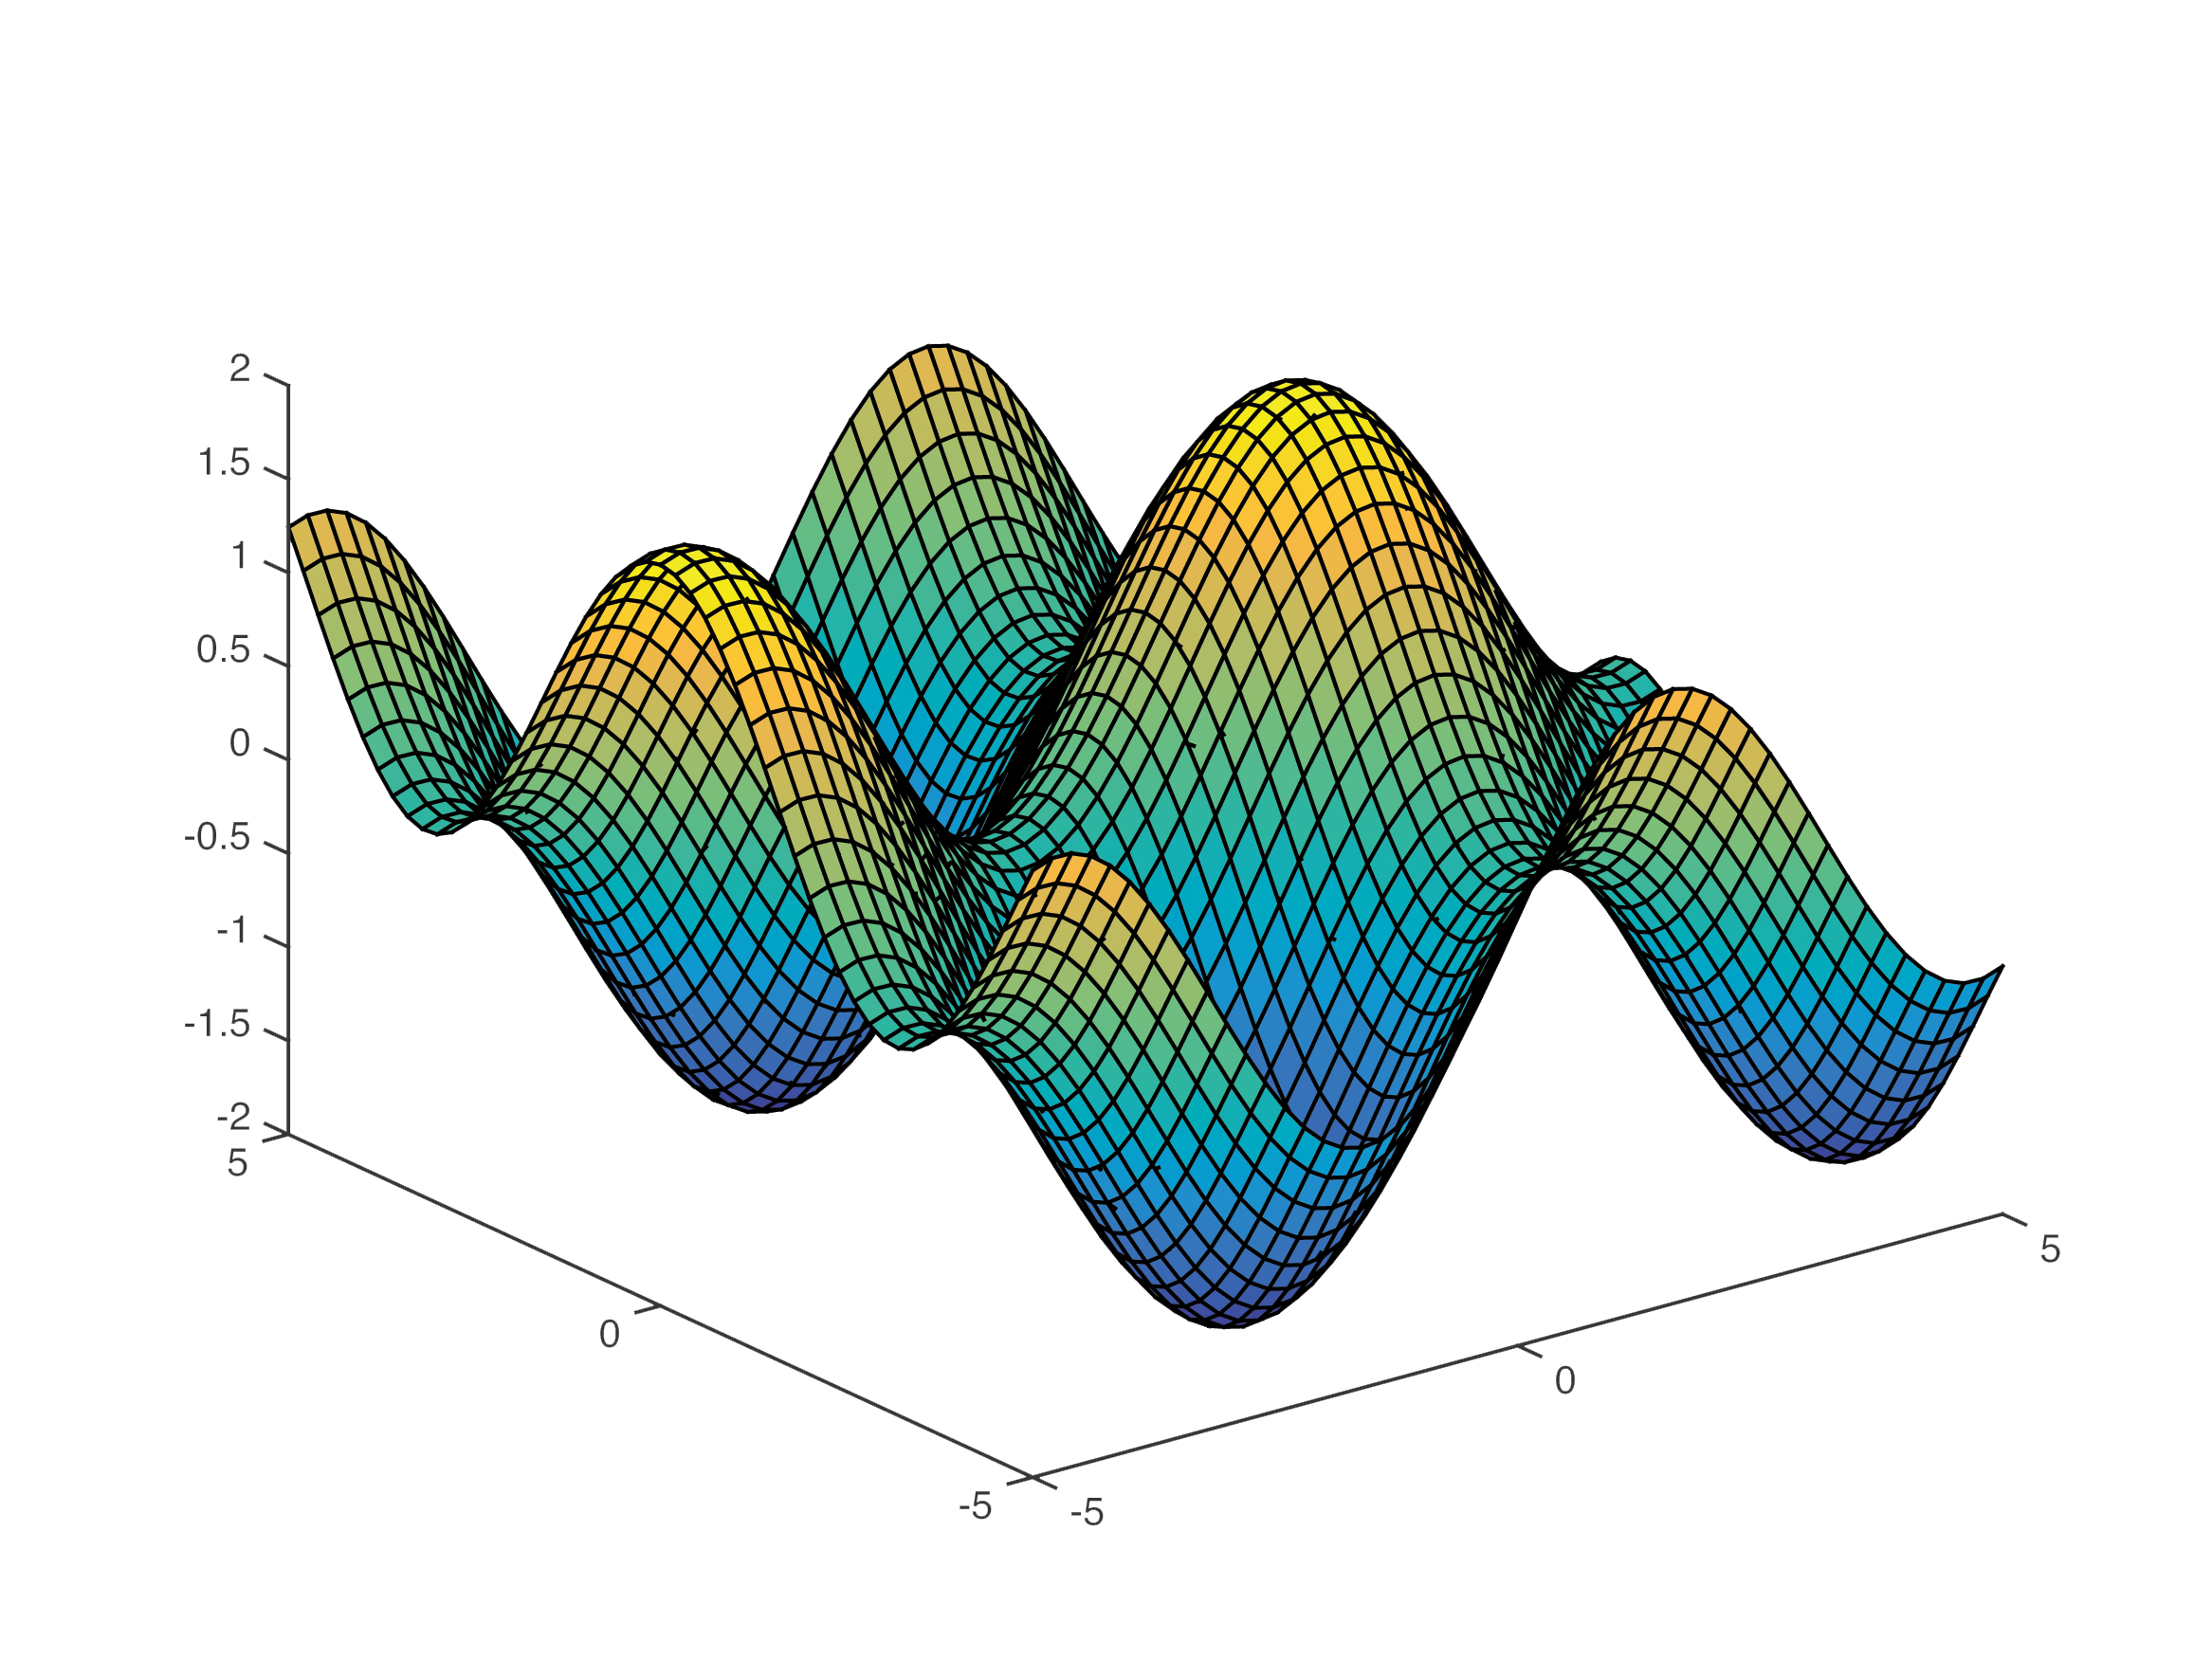
\includegraphics[scale=0.45]{figs/opt_function.png}	
		\caption{Exemplo de superfície da função $f(x,y)=sen(x)+cos(y)$.}
		\label{f.opt_function}
	\end{figure}
\end{frame}

\begin{frame}
	\begin{itemize}
		\justifying
		\item \textbf{Algoritmos} de Aprendizado de Máquina são usualmente \textbf{treinados} através de um processo de \textbf{otimização}~\cite{Lan:20};
		\\~\\
		\item Otimização permite o \textbf{ajuste de parâmetros} (variáveis) de acordo com o problema (\textbf{função de perda});
	\end{itemize}
\end{frame}

\begin{frame}
	\begin{figure}
		\centering
		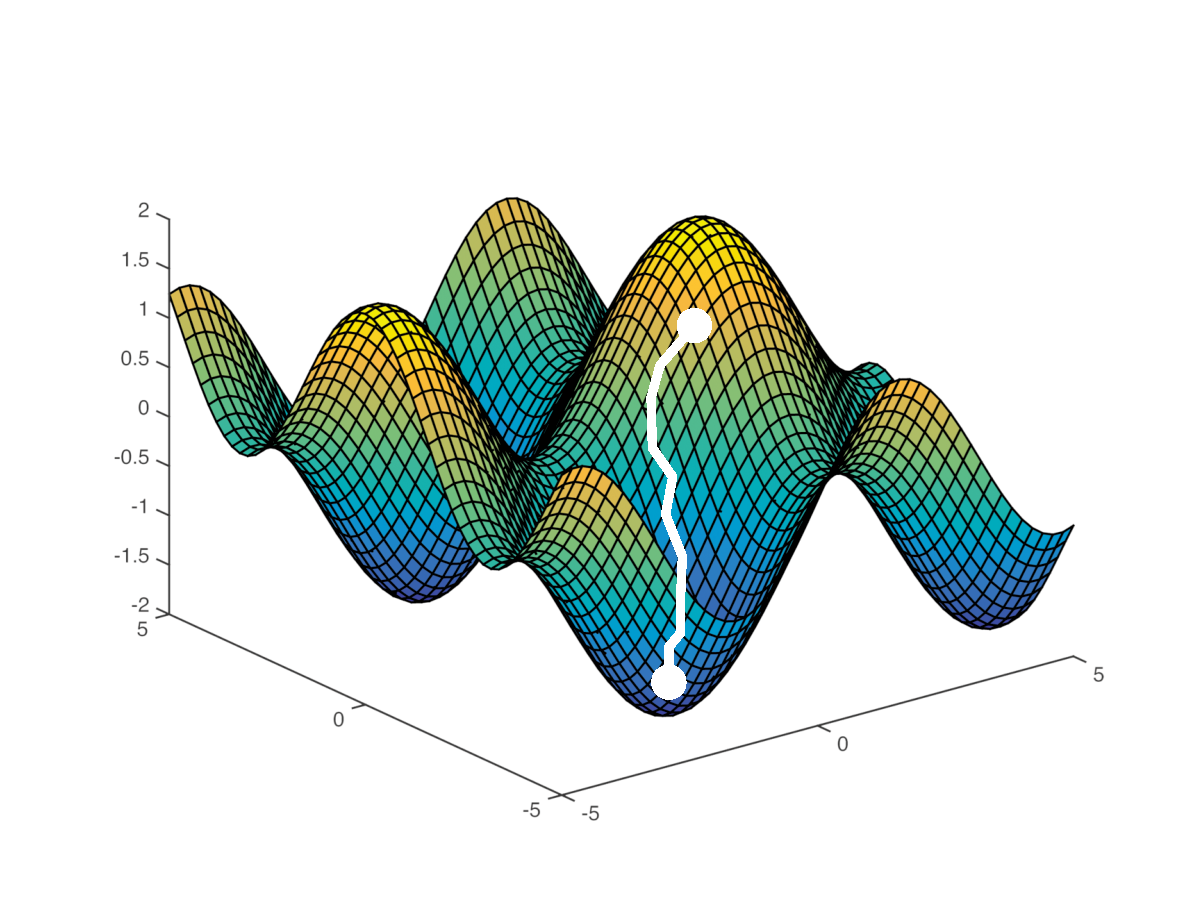
\includegraphics[scale=0.45]{figs/opt_function_opt.eps}	
		\caption{Exemplo de caminho realizado pelos passos da otimização até o encontro de um ponto de mínimo local.}
		\label{f.opt_function_opt}
	\end{figure}
\end{frame}

\subsection{Otimização Meta-Heurística}
\label{ss.optimization_mh}

\begin{frame}{Otimização Meta-Heurística}
	\begin{itemize}
		\justifying
		\item Modelagem matemática de \textbf{fenômenos da natureza} em algoritmos de \textbf{otimização}~\cite{yang_review};
		\\~\\
		\item \textbf{Heurísticas} (buscas) de \textbf{soluções} em espaços $n$-dimensionais;
		\\~\\
	\end{itemize}
	\vspace*{0.5cm}
	\begin{block}{}
		\centering
		\textbf{Diversificação} x \textbf{Intensificação}
	\end{block}	
\end{frame}

\begin{frame}
	\begin{figure}
		\centering
		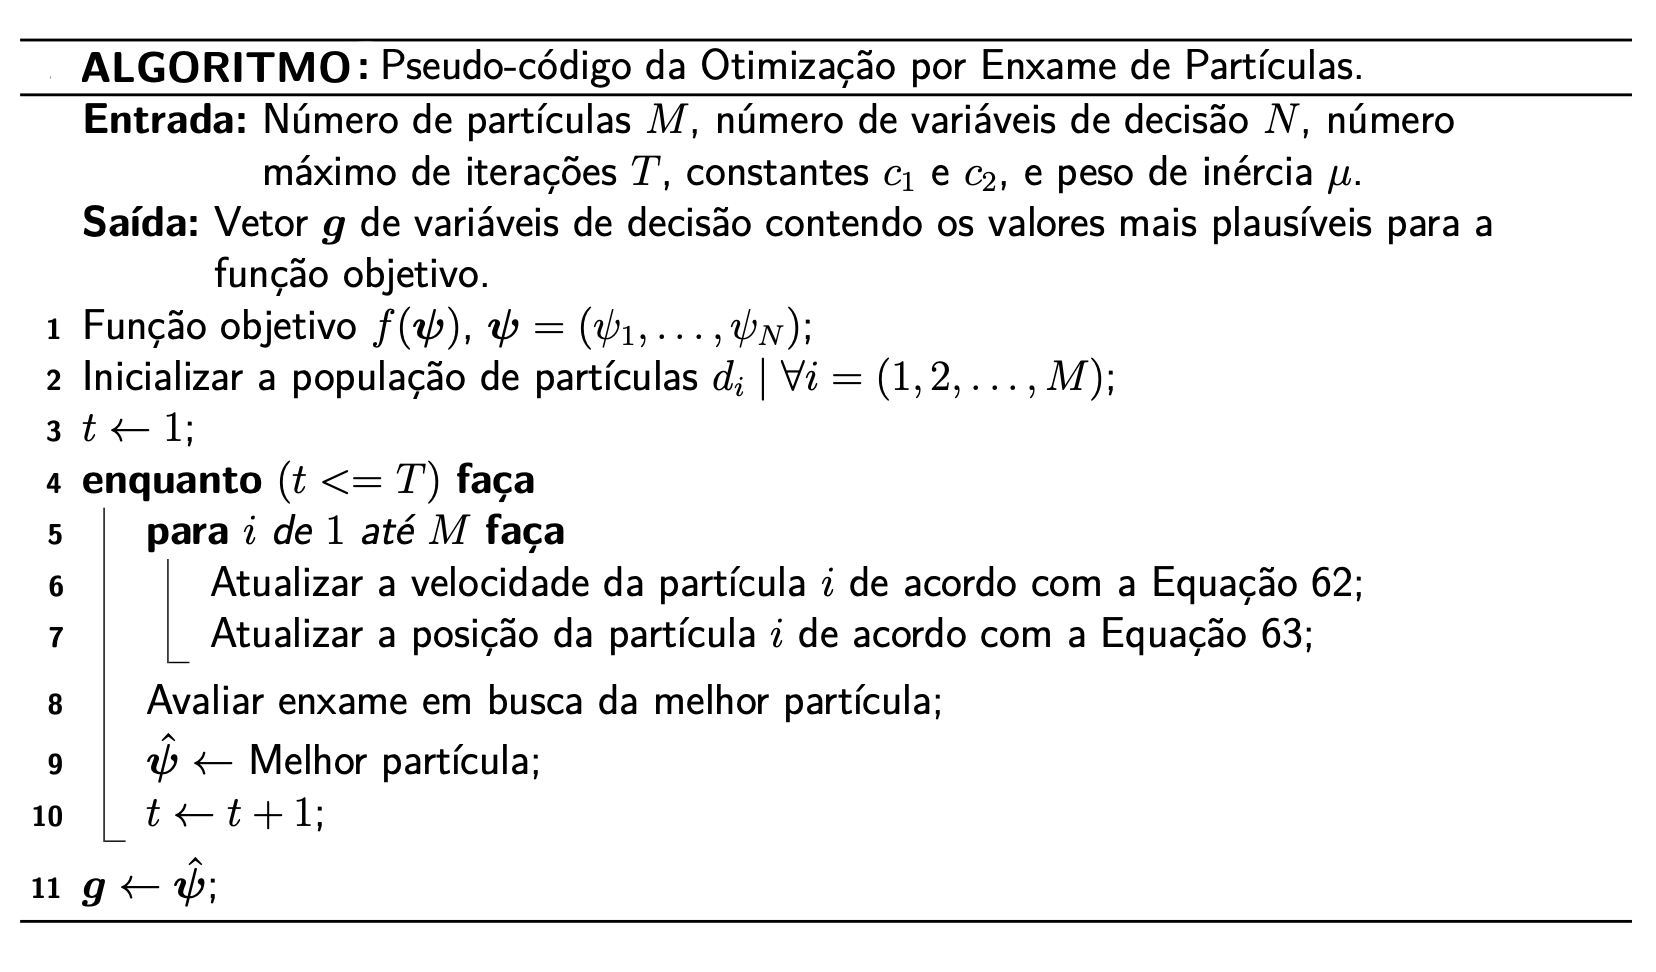
\includegraphics[scale=0.375]{figs/pso.png}	
		\caption{Pseudo-código da Otimização por Enxame de Partículas.}
		\label{f.pso}
	\end{figure}
\end{frame}